El Sol es una estrella que se ubica en la secuencia principal del diagrama \textit{Hertzsprung-Russell} (HR), de masa, luminosidad y temperatura efectiva promedio para nuestra galaxia. La gran diferencia esta en la posici�n que ocupara para los observadores terrestres. Por tanto, la cercan�a permite obtener im�genes de la superficie de este con mucha mayor resoluci�n espacial que la de cualquier otra estrella. Por otro lado, esta cercan�a hace que el flujo radiativo procedente de sol sea muy intenso. Estas dos condiciones anteriores permiten estudios simult�neos de alta resoluci�n espacial y tambi�n espectral~\cite{sunLibroAlberto}. 

El Sol tiene una composici�n de 70\% de Hidr�geno, 28\% de Helio y 2\% de elementos pesados, con un nucleo de densidad de 148000
kg/m$^3$, una edad aproximada de $4.6\times10^9$ a�os~\cite{cravens} y una estructura de capas como la mostrada en la Fig.~\ref{fig:solcapas}.

\begin{figure}
	\centering
	%Ruta
	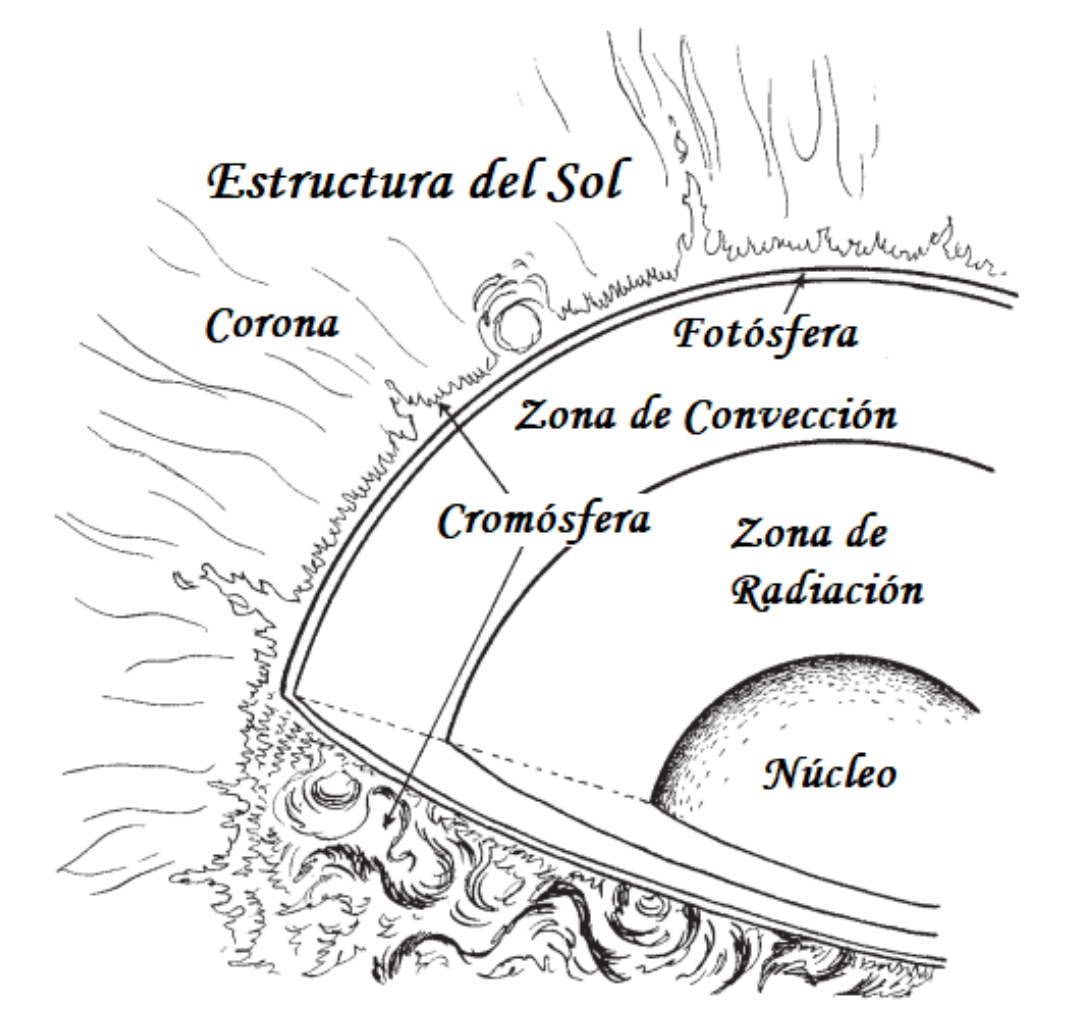
\includegraphics[width=0.8\textwidth]{./files/TFM/CAP04/figures/SolCapas.png}
	% caption
	\caption[]{Representaci�n de la estructura interna del Sol~\cite{garfinkle}.}
	\label{fig:solcapas}
\end{figure}

\section{Secci�n 1}
\label{sec:1cap2}



\subsection{Subsecci�n 1}



\subsection{Subsecci�n 2}


